% dibuix_cilindre_1.tex
\documentclass{standalone}
\usepackage{tikz}
\usetikzlibrary{arrows.meta, decorations.markings}

\begin{document}

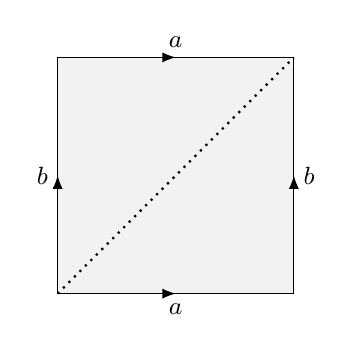
\begin{tikzpicture}[
    identified_edge/.style={
        decoration={
            markings,
            mark=at position 0.5 with {\arrow{Latex}}
        },
        postaction={decorate}
    },
    edge_label/.style={midway, auto, font=\small}
]

\def\squaresize{3}
\fill[gray!10] (0,0) -- (0,\squaresize) -- (\squaresize,\squaresize) -- (\squaresize,0) -- cycle;
\draw (0,0) rectangle (\squaresize,\squaresize);
\draw[dotted, thick] (0,0) -- (\squaresize,\squaresize);
\draw[identified_edge] (0,\squaresize) -- node[edge_label, above] {$a$} (\squaresize,\squaresize);
\draw[identified_edge] (0,0)       -- node[edge_label, below] {$a$} (\squaresize,0);
\draw[identified_edge] (0,0)       -- node[edge_label, left]  {$b$} (0,\squaresize);
\draw[identified_edge] (\squaresize,0) -- node[edge_label, right] {$b$} (\squaresize,\squaresize);

\end{tikzpicture}

\end{document}